\documentclass[notes,11pt, aspectratio=169]{beamer}
\usepackage[default]{lato}
%\usepackage{enumitem}
%\usepackage{color}
\newenvironment{transitionframe}{
  \setbeamercolor{background canvas}{bg=yellow}
  \begin{frame}}{
    \end{frame}
}


\setbeamercolor{frametitle}{fg=blue}
\setbeamercolor{title}{fg=black}
\setbeamertemplate{footline}[frame number]
\setbeamertemplate{navigation symbols}{} 
\setbeamertemplate{itemize items}{-}
\setbeamercolor{itemize item}{fg=blue}
\setbeamercolor{itemize subitem}{fg=blue}
\setbeamercolor{enumerate item}{fg=blue}
\setbeamercolor{enumerate subitem}{fg=blue}
\setbeamercolor{button}{bg=MyBackground,fg=blue,}
%\%setbeamercolor{block title}{fg=white,bg=blue}
%\setbeamercolor{block body}{fg=black,bg=gray}


% If you like road maps, rather than having clutter at the top, have a roadmap show up at the end of each section 
% (and after your introduction)
% Uncomment this is if you want the roadmap!
% \AtBeginSection[]
% {
%    \begin{frame}
%        \frametitle{Roadmap of Talk}
%        \tableofcontents[currentsection]
%    \end{frame}
% }
\setbeamercolor{section in toc}{fg=blue}
\setbeamercolor{subsection in toc}{fg=red}
\setbeamersize{text margin left=1em,text margin right=1em} 

\newenvironment{wideitemize}{\itemize\addtolength{\itemsep}{10pt}}{\enditemize}

%\documentclass[structure,compress,mathserif]{beamer}

\AtBeginSection[]{
  \begin{frame}
  \vfill
  \centering
  \begin{beamercolorbox}[sep=8pt,center,shadow=true,rounded=true]{title}
    \usebeamerfont{title}\insertsectionhead\par%
  \end{beamercolorbox}
  \vfill
  \end{frame}
}

\setbeamertemplate{caption}[numbered]
\usepackage{adjustbox}
\usepackage{threeparttable}
\usepackage{graphicx}
%\usepackage{chngcntr}
%\counterwithin{subfigure}{figure}
\usepackage{natbib}
\usepackage{float}
\usepackage{url}
\usepackage{hyperref}
\usepackage{color}
\usepackage{tabls, calc}
\usepackage[tableposition=top]{caption}
\usepackage{ifthen}
\usepackage{setspace}
\usepackage{booktabs}
\usepackage[english]{babel}
\usepackage[latin1]{inputenc}
\usepackage{caption}
\usepackage{subfigure}	
%\usepackage{custom}
\usepackage{tikz}
\usepackage{array}
\usepackage{dcolumn}
\usepackage{multirow}
\usepackage{markdown}
\usepackage{siunitx}
\usepackage{tfrupee}
%\usepackage[table]{xcolor}
%\usepackage{xcolor}
\usepackage{colortbl}
\usepackage{tcolorbox}

\tcbset{width=0.9\textwidth,boxrule=0pt,colback=red,arc=0pt,auto outer arc,left=0pt,right=0pt,boxsep=5pt}



%%%Define Colors Here
\definecolor{applegreen}{rgb}{0.55, 0.71, 0.0}
\definecolor{ao(english)}{rgb}{0.0, 0.5, 0.0}
\definecolor{pink}{rgb}{0.858, 0.188, 0.478}
\definecolor{purple}{rgb}{0.59, 0.44, 0.84}
\definecolor{denim}{rgb}{0.08, 0.38, 0.74}
\definecolor{seagreen}{rgb}{0.13, 0.7, 0.67}
\definecolor{tangerine}{rgb}{0.95, 0.52, 0.0}
\definecolor{textboxgreen}{rgb}{0.67, 0.88, 0.69}
\setbeamercolor{frametitle}{fg=denim}
%----------------------------------------------------------------------------------------
%	TITLE PAGE
%----------------------------------------------------------------------------------------
\title[DAR]{Data Analytics with R}  % The short title appears at the bottom of 
\author{Sumit Mishra} % Your name
\institute[IFMR] % Your institution as it will appear on the bottom of every slide, may be shorthand to save space
{
Institute for Financial Management and Research, Sri City \\ % Your institution for the title page
\medskip
\medskip
\textbf{Introduction to Data} % Your email address
}
\date{28 October 2020} % Date, can be changed to a custom date

%Preamble for ESTOUT
% *****************************************************************
% Estout related things
% *****************************************************************
\newcommand{\sym}[1]{\rlap{#1}}% Thanks to David Carlisle

\let\estinput=\input% define a new input command so that we can still flatten the document

\newcommand{\estwide}[3]{
		\vspace{.75ex}{
			\begin{tabular*}
			{\textwidth}{@{\hskip\tabcolsep\extracolsep\fill}l*{#2}{#3}}
			\toprule
			\estinput{#1}
			\bottomrule
			\addlinespace[.75ex]
			\end{tabular*}
			}
		}	

\newcommand{\estauto}[3]{
		\vspace{.75ex}{
			\begin{tabular}{l*{#2}{#3}}
			\toprule
			\estinput{#1}
			\bottomrule
			\addlinespace[.75ex]
			\end{tabular}
			}
		}

% Allow line breaks with \\ in specialcells
	\newcommand{\specialcell}[2][c]{%
	\begin{tabular}[#1]{@{}c@{}}#2\end{tabular}}

% *****************************************************************
% Custom subcaptions
% *****************************************************************
% Note/Source/Text after Tables
\newcommand{\figtext}[1]{
	\vspace{-1.9ex}
	\captionsetup{justification=justified,font=footnotesize}
	\caption*{\hspace{6pt}\hangindent=1.5em #1}
	}
\newcommand{\fignote}[1]{\figtext{\emph{Note:~}~#1}}

\newcommand{\figsource}[1]{\figtext{\emph{Source:~}~#1}}

% Add significance note with \starnote
\newcommand{\starnote}{\figtext{* p < 0.1, ** p < 0.05, *** p < 0.01. Standard errors in parentheses.}}

% *****************************************************************
% siunitx
% *****************************************************************
\usepackage{siunitx} % centering in tables
	\sisetup{
		detect-mode,
		tight-spacing		= true,
		group-digits		= false ,
		input-signs		= ,
		input-symbols		= ( ) [ ] - + *,
		input-open-uncertainty	= ,
		input-close-uncertainty	= ,
		table-align-text-post	= false
        }
%Preamble ends here 
%%%%%%%%%%%%%%%%%%%%%%%%%%%%%%%%%%%%%%%%%%%%%%%%%%%%%%%%%%%%%%%%%%%%%%%%%
%%%%%%%%%%%%%%%%%%%%%%%%%%%%%%%%%%%%%%%%%%%%%%%%%%%%%%%%%%%%%%%%%%%%%%%%%
              
\begin{document}
\begin{frame}
  \titlepage
\end{frame}

\begin{frame}{Agenda}
\begin{itemize}
\item Experiments Case Study: using stents to prevent strokes
\item Data basics.
\item Sampling principles and strategies.
\end{itemize}
\end{frame}


\section{Case: Stents to prevent strokes}
\begin{frame}{Using stents to prevent strokes}

\begin{figure}[h]
\centering
\begin{tabular}{l ccc}
\hline
Patient	&	group	&	0-30 days 	&	0-365 days \\
\hline
1		&	treatment &	no event &	no event \\
2		&	treatment &	stroke & stroke \\
3		&	treatment &	no event & no event \\
$\vdots$	&	$\vdots$	  &	$\vdots$ \\
450	&	control &	no event &	no event \\
451	&	control &	no event &	no event \\
\hline
\end{tabular}
\caption{Results for five patients from the stent study.}
\label{stentStudyResultsDF}
% trmt <- c(rep('trmt', 224), rep('control', 227)); outcome30 <- c(rep(c('event', 'no_event'), c(33, 191)), rep(c('event', 'no_event'), c(13, 214))); outcome365 <- c(rep(c('event', 'no_event'), c(33, 191)), rep(c('event', 'no_event'), c(13, 214)))
\end{figure}
\end{frame}

\begin{frame}{Using stents to prevent strokes}
\begin{figure}[h]
\centering
\begin{tabular}{l cc c cc}
& \multicolumn{2}{c}{0-30 days} &\hspace{5mm}\ & \multicolumn{2}{c}{0-365 days} \\
  \cline{2-3} \cline{5-6}
	& 	stroke 	& no event && 	stroke 	& no event \\
  \hline
treatment 	& 33		& 191	&&	45 	& 179 \\
control 		& 13		& 214	&& 	28	& 199 \\
  \hline
Total				& 46		& 405	&&	73	& 378 \\
  \hline
\end{tabular}
\caption{Descriptive statistics for the stent study.}
\label{stentStudyResults}
\end{figure}

\pause

Exercise: Calculate the proportion of people who had a stroke in the
treatment and control groups.
\end{frame}


\section{Data Basics}
\begin{frame}{Observations, variables, and data matrices}

Consider the following table.

\begin{figure}[h]
\centering
{\small
\begin{tabular}{ccc ccc cc} %c}
  \toprule \rowcolor{pink}
   & \texttt{loan\textunderscore{}amount}
   & \texttt{interest\textunderscore{}rate}
   & \texttt{term} & \texttt{grade} & \texttt{state}
   & \texttt{total\textunderscore{}income}
   & \texttt{homeownership} \\
  \hline \rowcolor{purple}
  1 & 7500 & 7.34 & 36 & A & MD & 70000 & rent \\
  2 & 25000 & 9.43 & 60 & B & OH & 254000 & mortgage \\
  3 & 14500 & 6.08 & 36 & A & MO & 80000 & mortgage \\
  $\vdots$ & $\vdots$ & $\vdots$ & $\vdots$ & $\vdots$ & $\vdots$
      & $\vdots$ & $\vdots$ \\
  50 & 3000 & 7.96 & 36 & A & CA & 34000 & rent \\
   \bottomrule
\end{tabular}
}
\caption{Four rows from the \texttt{loan50} data matrix.}
\label{loan50DF}
\end{figure}

\pause
\begin{columns}
\begin{column}{.5\textwidth}
\begin{minipage}[c][.3\textheight][c]{\linewidth}
\begin{wideitemize}
\small
\item Each row represents a single loan. 
     \begin{itemize}
     \item The formal name: \textcolor{purple}{observation}
     \end{itemize}
\pause
\item Each header represents characteristics of each loan.
      \begin{itemize}
      \item The formal name: \textcolor{pink}{variable}
      \end{itemize}
\end{wideitemize}
\end{minipage}
\end{column}
\hfill
\pause
%\begin{figure}
\begin{column}{0.48\textwidth}
\begin{minipage}[c][.2\textheight][c]{\linewidth}
\begin{wideitemize}
\item What does the first row represent?
     \begin{itemize}
     \item \textcolor{pink}{Loan amount}: \textcolor{purple}{\$ 7500}
     \item \textcolor{pink}{Borrower's location}: \textcolor{purple}{MD (Maryland)}
     \item \textcolor{pink}{Interest rate on the loan}: \textcolor{purple}{7.34\%.}
     \end{itemize}
\end{wideitemize}
\end{minipage}
\end{column}
%\end{figure}
\end{columns}

\end{frame}

\begin{frame}{Practice}

\begin{center}
Construct the gradebook for a course in \texttt{R} assuming that there are five students, two assignments, and one exam.
\end{center}
\end{frame}


\begin{frame}{Types of variables}
\begin{figure}[h]
  \centering
  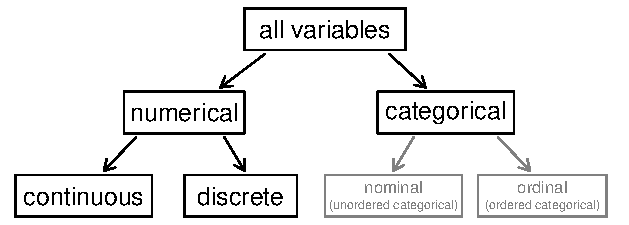
\includegraphics[scale=0.57]{graphs/variables.pdf}
  \caption{Breakdown of variables into their respective types.}
  \label{variables}
\end{figure}

\end{frame}


\begin{frame}{Relationship between variables}
\begin{center}
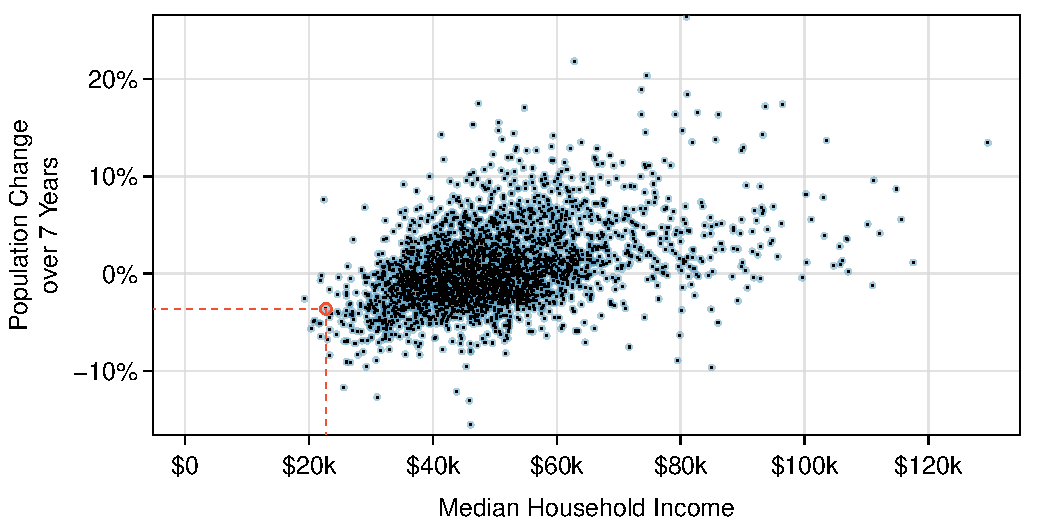
\includegraphics[scale=0.8]{graphs/pop_change_v_med_income.pdf}
\end{center}
\end{frame}

\begin{frame}{Practice}
Examine the variables in the \texttt{loan50} data set. Create two questions about possible relationships between variables in \texttt{loan50} that are of interest to you.
\end{frame}

\begin{frame}{Explanatory and Response Variables}
Think about the following question. \\

What will be the increase in \textcolor{seagreen}{sales} if there is a one percent rise in \textcolor{tangerine}{ad expenditure}? \\

\pause

The framing of the question is such that we seek a directional relationship between spending on ads and sales. 

\vspace{5mm}

\begin{center}

\colorbox{textboxgreen}{
$\texttt{Explanatory Variable} \Rightarrow \texttt{Response Variable}$
}

\end{center}
\end{frame}

\section{Sampling Principles and Strategies}

\begin{frame}{Introduction}
Consider the following possible responses to the three research questions:
\begin{itemize}
\item I subscribed to Spotify after I got tired of their annoying ads. Those annoying ads lead to greater number of subscriptions.
\item A student attending Random Coaching Classes was ranked first in the Pointless Entrance Exam. Therefore, on average, kids who attend Random end up in Pretentious Institute of Meritocracy.
\item An acquantaince who was infected with coronavirus was cured due to Coronil. Coronil is the cure for coronavirus.
\end{itemize}
\end{frame}

\begin{frame}{Sampling from a population}

Objective: Estimate the time to graduation for university undergraduates in the last five years by collecting a sample.
\begin{center}
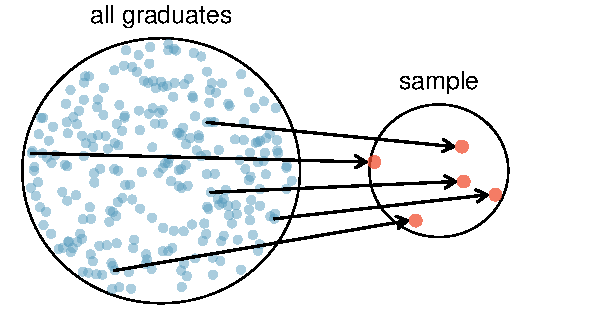
\includegraphics[scale=0.8]{graphs/popToSampleGraduates}
\end{center}

\end{frame}


\begin{frame}{Sampling from a population: Example}

Let's suppose that a student from medicine is being asked to select survey respondents and he ends up oversampling other students from his own field. This introduces a \textbf{bias}.
\begin{center}
\includegraphics[scale=0.8]{graphs/popToSubsampleGraduates}
\end{center}

\end{frame}


\begin{frame}{Simple random sample}

To avoid the problem that we saw in the previous slide, we will employ a simple random sample. \\

\vspace{5mm}

\pause

This means that each person in the population has an equal chance of being included. 

\vspace{5mm}
\pause

Even after having chosen the sample carefully, some people may choose not respond. This introduces another form of bias known as the \textbf{non-response bias}.
\begin{center}
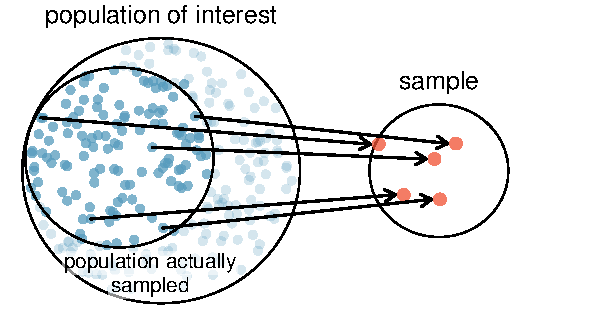
\includegraphics[scale=0.8]{graphs/surveySample}
\end{center}

\end{frame}

\begin{frame}{Sampling Methods}
\begin{figure}
\centering
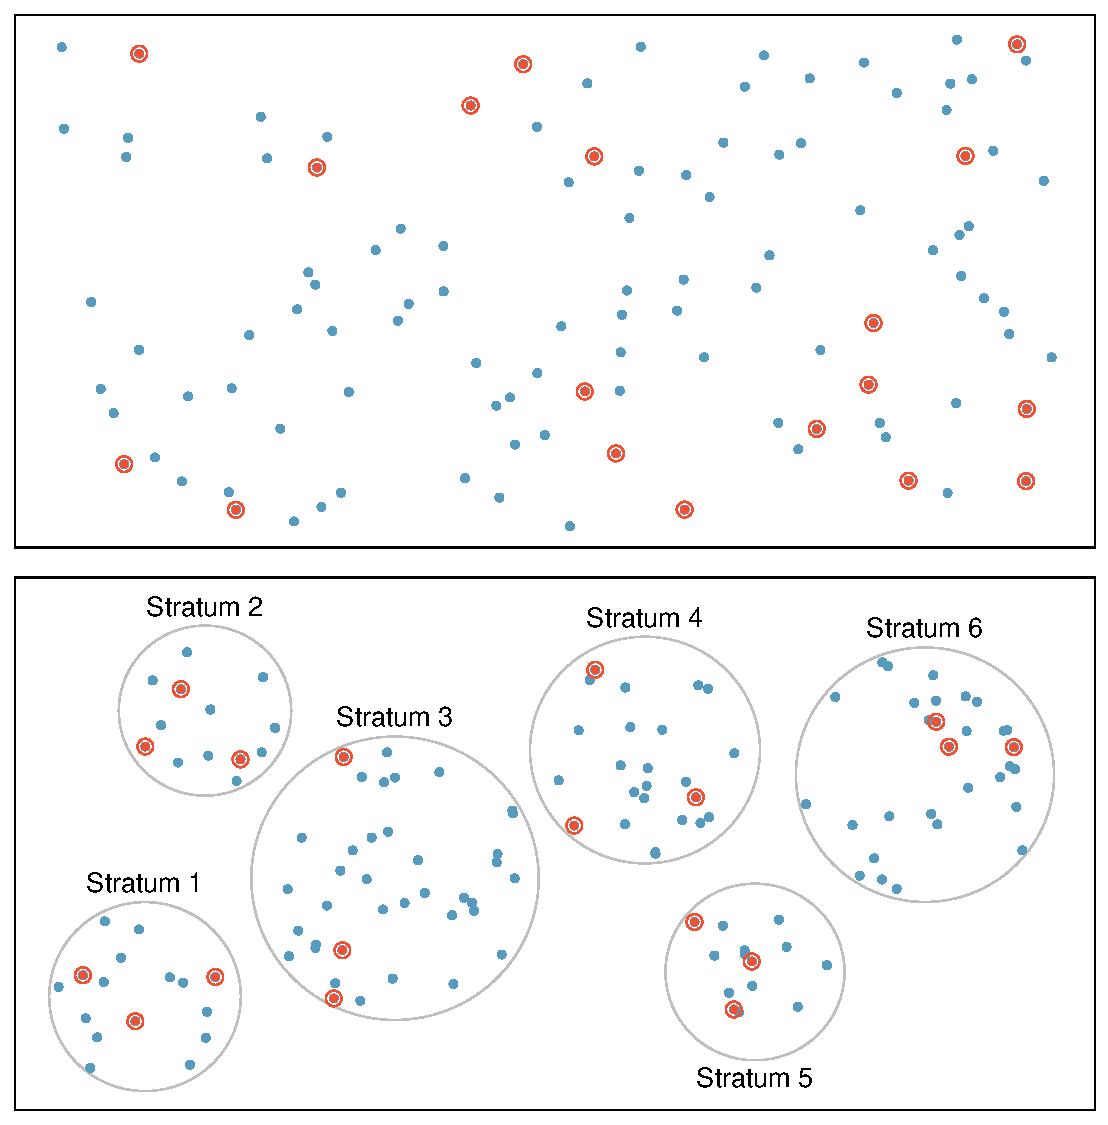
\includegraphics[scale = 0.3]{graphs/simple_stratified}
\caption{Examples of simple random\index{sample!simple random sampling} and stratified sampling\index{sample!stratified sampling}. In the top panel, simple random sampling was used to randomly select the 18 cases. In the bottom panel, stratified sampling was used: cases were grouped into strata, then simple random sampling was employed within \mbox{each stratum}.}
\label{simple_stratified}
\end{figure}

\end{frame}


\begin{frame}{Sampling Methods}

\begin{itemize}
\item \textbf{Simple random sampling}
     \begin{itemize} 
      \item Example: You want to estimate salaries of IPL players (there are eight IPL teams).
      \item Let's assume that there are 160 players, and you are going to sample 16 of them.
      \item You write the names of the players onto slips of paper.
      \item Randomly pick 16 players.
      \end{itemize}

\pause
\item \textbf{Stratified sampling}
     \begin{itemize}
     \item You will choose two players from each team (randomly of course).
     \item This is especially useful when the observations in each \textit{stratum} are very similar.
     \end{itemize}
\end{itemize}
\end{frame}

\begin{frame}{Sampling Methods}

\begin{itemize}

\item \textbf{Cluster sample}:
       \begin{itemize}
       \item Break up the population into many groups.
       \item Choose a fixed sample of clusters.
       \item Survey all observations from each of these clusters.
       \end{itemize}

\pause
\item \textbf{Multi-stage sample}
      \begin{itemize}
      \item Random sampling within each cluster.
      \end{itemize}
\end{itemize}

These approaches are useful when clusters are largely similar, but there's lot of variation within each of these clusters.

\end{frame}

\begin{frame}{Sampling Methods}
\begin{columns}
\begin{column}{.5\textwidth}
\begin{minipage}[c][.6\textheight][c]{\linewidth}
\begin{figure}
  \centering
  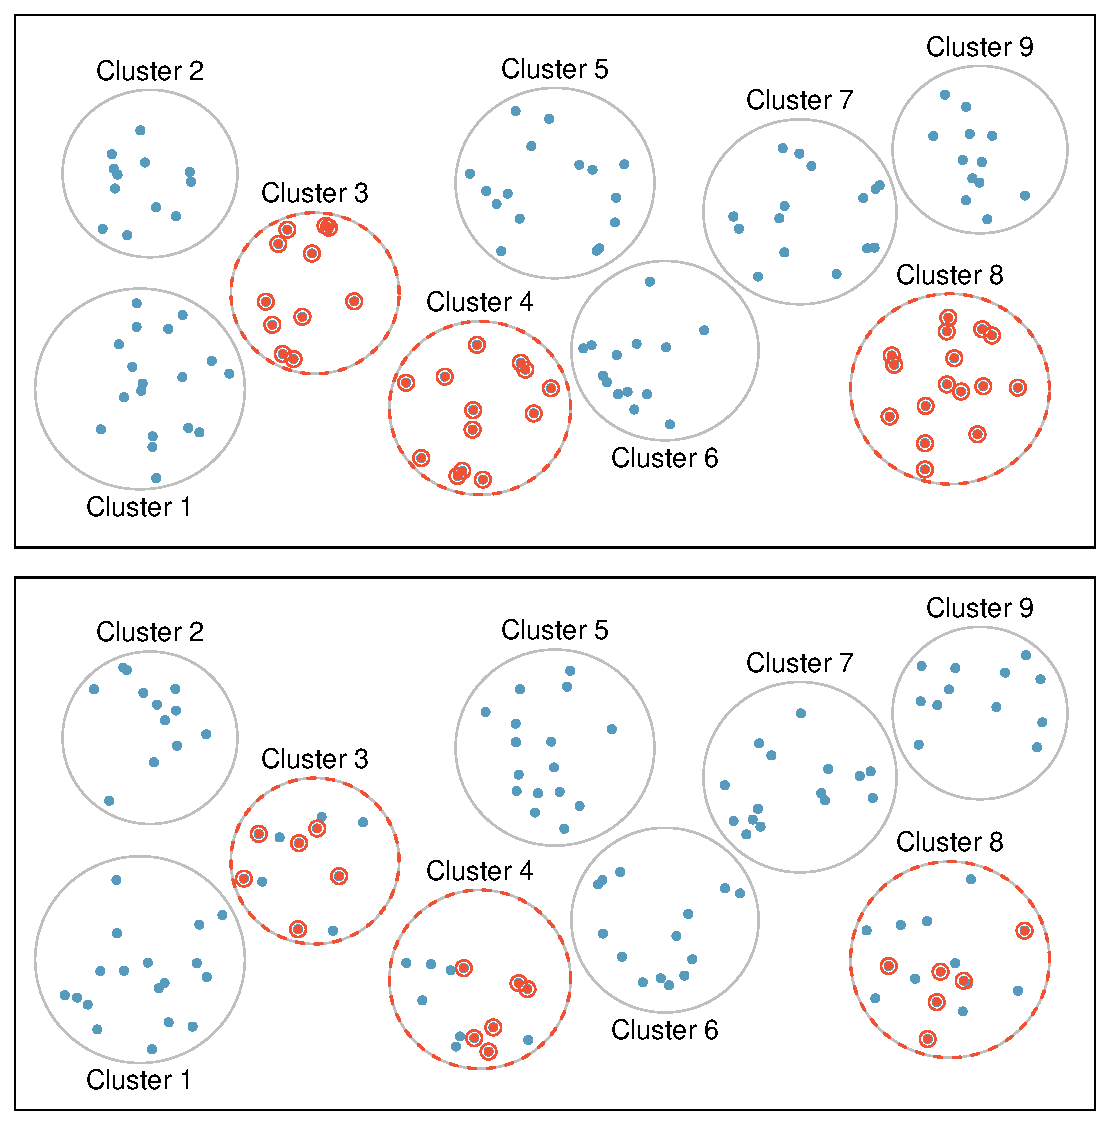
\includegraphics[scale=0.35]{graphs/cluster_multistage}
 \label{cluster_multistage}
\end{figure}
\end{minipage}
\end{column}

\hfill
\begin{column}{.5\textwidth}
\begin{minipage}[c][.6\textheight][c]{\linewidth}
\begin{itemize}
\item \textbf{Cluster sampling (Top Panel)}
        \begin{itemize}
        \item Data binned into 9 clusters.
        \item 3 out of 9 were sampled.
        \item Everyone in those 3 clusters were sampled.
        \end{itemize}
\item \textbf{Multistage cluster sampling (Bottom Panel)}
        \begin{itemize}
        \item Randomly select three clusters.
        \item Randomly draw people from each of these clusters.
        \end{itemize}
\end{itemize}
\end{minipage}
\end{column}
\end{columns}

\end{frame}

\end{document}